\newpage
\thispagestyle{sectioned}
\chapter{Technologies and Methods}
%\addcontentsline{toc}{chapter}{\numberline{Technologies and Methods}}
This chapter will explain all of the technologies and techniques that have been used and applied to finish this work.
\section{Technologies}
Multiple utilities for a wide variety of purposes have been used. Some of them such as the choice of web server or Integrated Development Environment are alternatives selected for their personal perception of fitness to the task to solve. Others such as Wave and the Google Web toolkit are essential and irreplaceable.
\subsection{Wave}
Wave can be interpreted as different things: The project formerly known as Google Wave and now Apache Wave, the system Wave In A Box which is the main focus of the Apache Wave project, the communication protocol inside Wave In A Box created by Google for \textbf{human comunication} and inspired in email, or one of the units of communication inside this protocol. In the making of this work every extension has been developed and tested under two varieties of Wave: Wave In A Box and Kune \cite{ref:kune}. Kune nowadays has much of its code forked from the Wave In A Box repository, but adding more functionality around it or changing it. Gadgets and apps are built into the core of Wave, and, as such, Kune inherits all their capabilities, making the gadgets and robots explored here compatible with both technologies. The people behind Kune are Colectivo Comunes \cite{ref:comunes}, a non-profit collective that tries to help other collectives to carry their operations by developing some web tools and free resources.
\begin{figure}[H]
  \center
    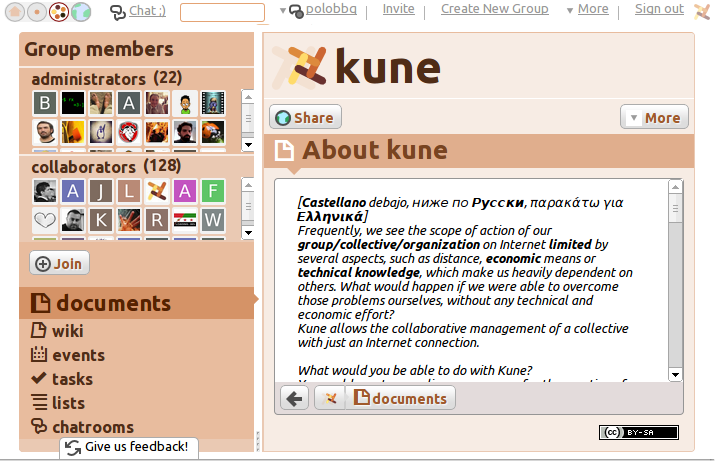
\includegraphics[keepaspectratio, scale=0.26]{Media/Captures/Wave/Kune_Groups.png}
  \caption{Kune Groups}
  \label{fig:kune_groups}
\end{figure}
The main technical feature that characterizes Wave is the \textbf{Wave Federation Protocol} \cite{ref:wave_federated_protocol}, that handles all of the communication happenning between users. It is an esxtension of the Extensible Messaging and Presence Protocol \cite{ref:xmpp} that adds federation on top of it. Wave being an open protocol allows anyone to be a Wave provider, Participants send delta changes on the content, and those deltas are distributed through the rest of the participants, guaranteeing that the end result is the same for everyone \cite{ref:federating_websites_google_wave}. Gadgets and robots will work under this environment, interacting with the Wave protocol.

\subsection{Google Web Toolkit}
Google Web Toolkit \cite{ref:gwt}, or GWT, is a set of tools that allows web developers to code in Java and from that java-compliant code, generate Asynchronous JavaScript and XML (AJAX) code to make front-end applications. The GWT framework focuses on efficiency and cross-browser compatibility, generating \textbf{AJAX from Java code} and then serving different compilations for every browser and locale combination, so the elements are rendered as they should in each browser, even though they behave differently. GWT provides the developer with all the common web controls, allows RPC invokations, browser history management, unit testing, and native JavaScript calls, among other features.
\begin{figure}[H]
  \center
    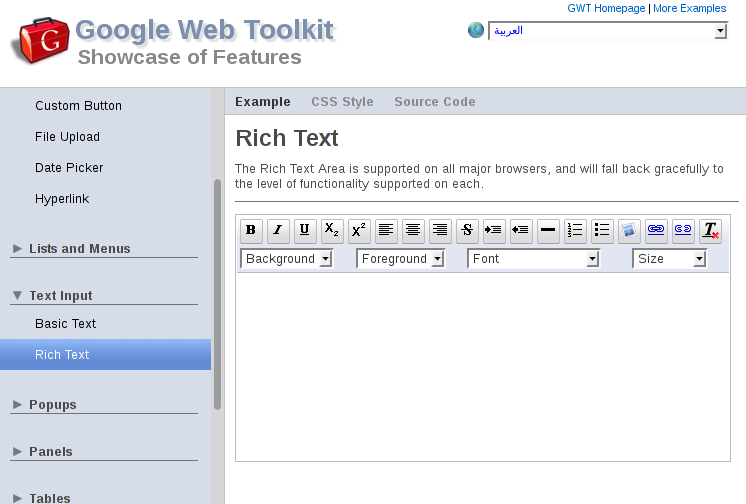
\includegraphics[keepaspectratio, scale=0.4]{Media/Captures/GWT/gwt_showcase.png}
  \caption{GWT Showcase}
  \label{fig:gwt_showcase}
\end{figure}
GWT has a development mode, where the Java code is not compiled to JavaScript, but instead it is ran in native Java and simulates the JavaScript components that will be used later. The development mode also allows a Java debugger to attach to GWT and debug the application locally. 

\subsection{Gadgets API}
The Gadgets API \cite{ref:gadgets_api} is made by Google to \textbf{embed third party applications inside various Google products}. They implemented it in wave as Wave Gadgets API, to have access to the specific features of Wave. These applications are HTML and JavaScript, with all their possibilities, and access specific features that the server can offer.\\[.2cm]
This is a Java API, and it needs to be compiled with the GWT compiler in order to be able to link to the gadgets. Apart from being able to use all GWT components, this API lets the developer communicate with Wave, and that means mainly altering the state and responding to state changes. The state contains the participants, and the content, plus more information.

\subsection{Robots API}
The Robots API \cite{ref:robots_api} is an API with client libraries for Java an Python, both of them implementing the same set of features. The original intention was to make \textbf{robots able to act in Wave like human participants} and in exactly the same places and same ways as actual participants could. In practice, not all interactions are implemented for robots. A robot can be added to a Wave, can edit text, add participants, publish new Wavelets, and access the contents of all of them, as well as responding to events about changes in the document or participants.

\subsection{Other Technologies}
Also worth mentioning are the following technologies:
As an IDE Eclipse \cite{ref:eclipse} 3.8 has been used for developing the gadgets as well as the robot. OpenJDK \cite{ref:openjdk} 7 has been used as Java Development Kit. Jetty \cite{ref:jetty} 6.1.24 has been used for a local robot server. Tomcat7 \cite{ref:tomcat} along with Shindig have been used as a local gadget server. Chromium \cite{ref:chromium} 32 and Iceweasel \cite{ref:iceweasel} 24.3 have been used for testing the results. Maven \cite{ref:maven} has been used for dependency management. The service Appear.in has been used to make the video interaction in the Video Conference Gadget. The Java library google-diff-match-patch has been used to calculate diffs between texts for creating the Colorizer Robot. Vaadin's GWT Graphics library has been used in the Decision Maker Gadget to draw some of its interface. Figure \ref{fig:logos} shows the logos of most of the technologies used. Table \ref{fig:technologies} shows a selection of technologies along with their purpose.
\begin{figure}[h]
  \center
    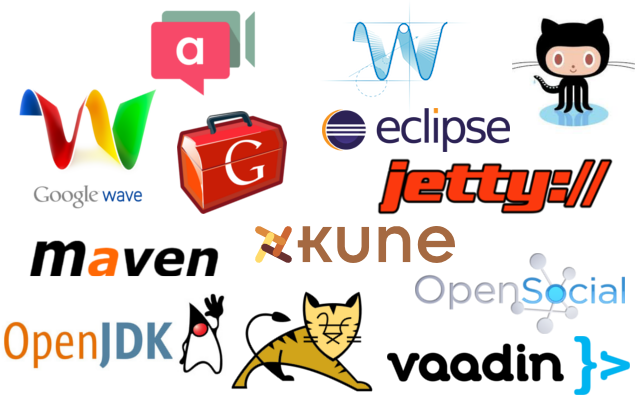
\includegraphics[keepaspectratio, scale=0.45]{Media/logos.png}
  \caption{Technologies Used}
  \label{fig:logos}
\end{figure}
\begin{table}[h]
  \footnotesize
  \begin{center}
    \begin{tabular}{ | c | c | c |}
      \hline
      \textbf{Type} & \textbf{Name} & \textbf{Use}\\
      \hline
      \multirow{2}{*}{APIs}
        & Robots API & Creating Java Robots for Wave \\ \cline{2-3}
        & Gadgets API & Creating Gadgets for Wave \\
      \hline
      \multirow{3}{*}{Servers}
        & Tomcat & Web server for storage \\ \cline{2-3}
        & Shindig & Gadgets server with OpenSocial support \\ \cline{2-3}
        & Jetty & Java server for robots \\
      \hline
      \multirow{2}{*}{Wave}
        & Wave In A Box & Testing Robots and Gadgets \\ \cline{2-3}
        & Kune & Testing Robots and Gadgets, documenting \\ \cline{2-3}
      \hline
      \multirow{3}{*}{Libraries}
        & Appear.in & WebRTC video communication \\ \cline{2-3}
        & Google diff-match-patch & Calculating differences between two texts \\ \cline{2-3}
        & GWT Graphics & Drawing shapes in GWT \\
      \hline
    \end{tabular}
  \end{center}
  \caption{Technologies Summary}
  \label{fig:technologies}
\end{table}

\section{Methods}
This chapter will explain the different techniques and decisions used and taken to successfully meet all the requirements and approach the problems trying to be as close to the software engineering process as possible. There has been a special focus on open source, standards and patterns.
\subsection{Free Open Source Software Approach}
Everything here such as this report, and the whole code has been \textbf{developed openly} and released under a relatively restrictive copyleft license. A Github Organization is a conglomerate of organized software repositories stored together and hosted on github.com. The progress, as well as the code, can be visited at the following Github Organization:
\begin{center}\url{https://github.com/End-of-degree-project}\end{center}
The license chosen for the software is the \textbf{AGPL}, which is an extension of GPL. GPL basically affects distribution of derivative works, forcing the distributor to provide the source code of everything and distribute it with the same license. AGPL has the same restriction, but extends GPL by also forcing the code to be published under the same license, even if the derivated work is not distributed.\\[.2cm]
It is important to observe that open source and open development are not related one to another. Although sources differ when defining what open source is, they all basically agree that source of the software should be available, and some liberties of use, modification and distribution are given to the users. This project is open source, but it has also been developed openly. That means the evolution of the work as well as the one of this document can be seen in the commits of the repositories. Collaboration would have also been accepted, and issues attended.
\subsection{Standards \& Protocols}
Open source software and free protocols have been used when possible. That improves the visibility of the project and increases the chance of it being reused, modified, and useful even for the purpose of other people.\\[.2cm]
\textbf{OpenSocial} \cite{ref:opensocial}: They efficiently descibe themselves ``OpenSocial Gadgets are a mechanism for embedding one web application into other web application using modern Javascript and HTML5 technology''. They basically are a standard that make gadget implementation possible, it is a public specification of various procedures to create a ``hosting environment'', understanding that as a web container that can house other elements.\\[.2cm]
\textbf{Wave Federation Protocol} \cite{ref:wave_federation_protocol}: Again, a good definition is the one given to themselves as ``a server-to-server network protocol between service providers, supporting low-latency, concurrent updates to conversations (live typing) and domain authentication''. But the most relevant aspect for Wave is that it provides federation, which again in their own words is ``The utility of waves is greatly enhanced if they can be federated in the sense that they are shared between users from different organisations, hosted by different service providers across the Internet''.\\[.2cm]
Much more information can be found on the Google Wave Federation White Paper \cite{ref:wave_white_paper} and the Draft Protocol Specification \cite{ref:wave_over_xmpp}.\\[.2cm]
Also, the structures have been planned and modelled beforehand in UML \cite{ref:uml} in order to be implemented later. \textbf{UML diagrams} can be found in the Table of Figures with the prefix \verb|UML|.
\subsection{Patterns}
The Model View Controller pattern has been followed in every gadget when interacting with with the GWT components. The Model View Controller makes use of object orientation to divide a software application to separate the internal representation of the software from the way it is shown to the user.\\[.2cm]
The Observer pattern has been implemented in all the gadgets in order to wait and answer to state changes on the Wave's state. In this pattern an object, called the subject, holds a list of other dependent classes called observers. When a state change that wants to be notified happens on the subject, it will notify the observers of the change.\\[.2cm]
Use of the Dependency Injector has been carried out by using GIN in both the gadgets and the robot to satisfy dependencies in an inverse order \cite{ref:dependency_injection}. This pattern implements the dependency inversion principle, to make high-level modules not dependent on low-level elements, exactly the oposite as the traditional dependency pattern. To achieve it the dependencies are passed by reference to the dependent object. Using GIN or Guice makes this process very simple.

\subsection{Extensions}
Both possible ways for extending Wave have been explored in this work. Gadgets have been implemented with the Wave Gadgets API, and robots with the Java version of the robots API.
\begin{figure}[h]
  \center
    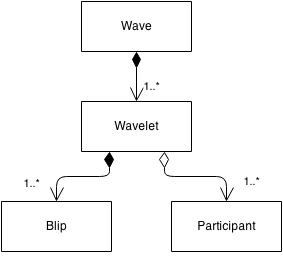
\includegraphics[keepaspectratio, scale=0.7]{Media/Diagrams/Wave/Structure.png}
  \caption{UML Class Diagram, Wave Structure}
  \label{fig:wave_structure}
\end{figure}
To understand where these extensions live, it is necessary to understand how wave is structured. In Figure \ref{fig:wave_structure} you can see \textbf{how Wave documents are structured}. The outermost layer is the wave, a thread or conversation, the whole picture of a conversation. Users are invited to the wave, letting them participate in any of the inner wavelets, when they then become participants. As of today, in current versions of Wave In A Box and Kune, there is only one wavelet inside every wave, but the Wave Protocol allows for multiple wavelets. \textbf{Blips are individual messages created by a participant}, and edited by participants later. Blips have hierarchical structure and can be nested inside other blips. Blips also contain a document in XML-like format, which is the text itself plus all the variations that Wave supports such as annotations.

\chapter{Frame for Development of Gadgets \& Robots}
As stated before, there is an important lack of documentation affecting anything relating to Wave. Through the progression of this project some obstacles, and the following chapter describes how they can be overcome. In addition to that, it explains the structure followed to implement the extensions as well as the operation of part of the features in Wave.
\section{Gadgets}
As explained before, gadgets are applications by themselves, but depending on some bigger entity, in this case the Wave server. Gadgets are inserted inside a document, together with the content itself. They are \textbf{placed inside a blip}, but belong to the wave and therefore have access to the whole wave's content, wich is given access by the Gadgets API. But that access is very limited, almost only to access what is called the wave's state, a key-value dictionary that keeps track of every state change that occurs inside the wave.\\[.2cm]
There is actually two differentiated kind of states in a wave:
\begin{itemize}
  \item \textbf{Private State}: stores information that can only be accessed and modified from the participant that created it. Useful to keep stored private information that is not intended to be shared.
  \item \textbf{Shared State}: stores the global state of every gadget in this wave, representing the whole picture. Useful for communicating with the other participants and collaborating or comunicating in the gadget.
\end{itemize}
It is important to know that the state belongs to the wave, so gadgets will have access to the other gadgets state, even different instances of the same gadgets. It is then good practice to adopt a system similar to namespaces in programming languages, appending an identifier of the gadget before the key in a way we are not altering or reading an unintended state.\\[.2cm]
Each actual instance of the gadget in a participant's browser is local, \textbf{variables are not shared} in any way between different participants. When a user triggers a state change in his local instance of the gadget, the only thing that can be communicated outside of the browser is a delta, that is an addition, deletion or modification in the key-value pairs that represent the state. This delta is then communicated to the local instance of the gadget in every client's browser so they can act accordingly and represent the new state. That behaviour can be seen illustrated in figure \ref{fig:wave_state}.
\begin{figure}[H]
  \center
    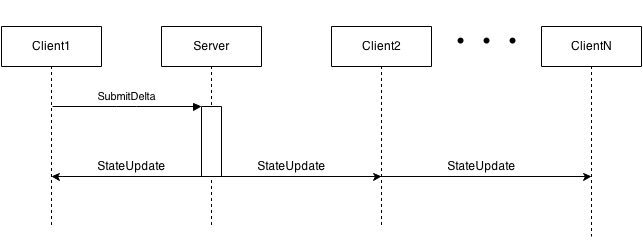
\includegraphics[keepaspectratio, scale=0.6]{Media/Diagrams/Wave/StateSequence.png}
  \caption{UML Sequence Diagram, Wave state transmission}
  \label{fig:wave_state}
\end{figure}
The Gadgets API asks you to follow a class hierarchy in order to be able to correctly communicate with wave. That hierarchy is as seen in Figure \ref{fig:gadget_classes}.\\[.2cm]
\begin{figure}[h]
  \center
    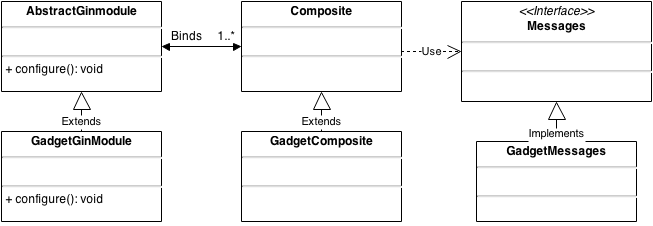
\includegraphics[keepaspectratio, scale=0.5]{Media/Diagrams/Gadget/Gadget.png}
  \caption{UML Class Diagram, Gadgets API class structure}
  \label{fig:gadget_classes}
\end{figure}
Those classes will interact in the following way:
\begin{itemize}
  \item AbstractGinModule: GIN is Guice for GWT client-side code, built on top of Guice and with a subset of Guice binding language. It allows the programmer to follow the pattern of dependency injection. This module attaches all of the modules together.
  \item Composite: Is the actual visual representation of the gadget. This is a GWT class ideated for creating custom widgets. Composites can contain a panel, and inside the panel complex GWT component hierarchies can be built. All features of GWT are supported thanks to this component.
  \item Messages: A GWT interface meant to be implemented by a class that gives access to the strings needed to build the interface. Those strings can be localized to make the gadget available in different languages for each client. The locale is determined by the Accept-Language field in the browser's HTTP request \cite{ref:gwt_internationalization} and served at runtime to the browser. Typically this class will be used from the Composite, or any of its inner components, to fill them with human-readable language.
\end{itemize}
With every one of the gadgets there is available a \textbf{tester and a deployer}, both of them depending on the main gadget, which is common for both.
\begin{figure}[H]
  \center
    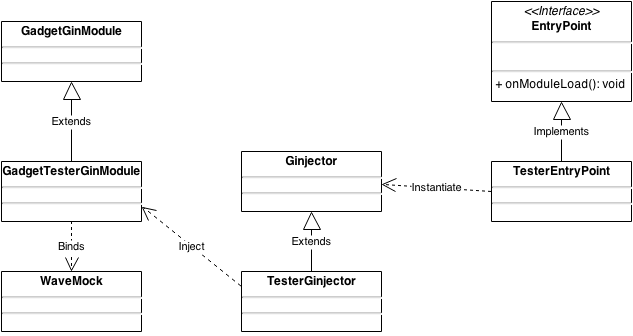
\includegraphics[keepaspectratio, scale=0.5]{Media/Diagrams/Gadget/Tester.png}
  \caption{UML Class Diagram, Gadget Tester Structure}
  \label{fig:gadget_tester}
\end{figure}
The tester project seen in Figure \ref{fig:gadget_tester} shows the common class hierarchy used in every one of the \textbf{tester projects}, which makes use of the development mode available in GWT, so gadgets can be quickly tested before deploying them. It is linked to the one seen in Figure \ref{fig:gadget_classes} by the GadgetGinModule, whis is inherited by the GadgetTesterGinModule. This new Gin module adds another injection, the WaveMock. This is a mock class that \textbf{simulates the basics of the behaviour of the Wave infrastructure} without the need to deploy the whole Wave system. To complete the needs of GIN a class extending Ginjector is created, the TesterGinjector, whose task is to actually inject the GinModule. This injector is instantiated inside a class that implements the interface EntryPoint that, as its name says, will be the entry point of our gadget in the onModuleLoad method. This project has to be run as a Web Application with Google's App Engine.
\begin{figure}[H]
  \center
    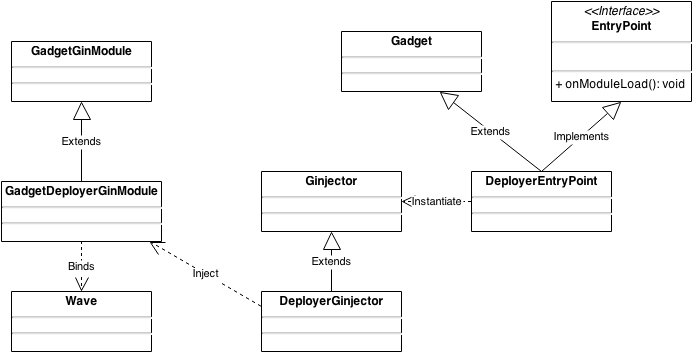
\includegraphics[keepaspectratio, scale=0.5]{Media/Diagrams/Gadget/Deployer.png}
  \caption{UML Class Diagram, Gadget Deployer Structure}
  \label{fig:gadget_deployer}
\end{figure}
The \textbf{deployer project} represented in Figure \ref{fig:gadget_deployer} is the project used to generate all the final JavaScript files ready to deploy to a web server with support for gadgets. An intermediate XML file containing JavaScript code is generated with enough logic to figure out which one of the browser and locale configuration has to be served.\\[.2cm]
It is very similar to the tester organization but with two basic differences. First, the GadgetGinModule now binds the class Wave instead of a Wave mock, as it will be running in the \textbf{whole Wave environment}. The other difference is that the EntryPoint, as well as implementing the same interface as before, now also extends the Gadget class, coming from the Gadgets API and representing a gadget. This project needs to be GWT compiled to succesfully generate all the files.\\[.2cm]
Gadgets have been tested for deployment using Tomcat as a web server and Shindig as a gadgets server with support for OpenSocial. Several files are generated after GWT compiling, and they should all be put together in the same directory and accessible from outside the own server. Shindig is then deployed as an application inside Tomcat.\\[.2cm]
Shindig needs to be configured accordingly:
\begin{itemize}
  \item First add ``wave'' to the gadgets.container in the \verb|container.js| file, in order to support Wave. As Wave does not use security token (OAuth's authentication token) for gadgets, you have to set Shindig not to require it by adding the following line: \verb|``render_token_required'' : false,|.
  \item Then you have to instruct Wave to use the gadgets server that was configured. The place to do that is a file called server.config in Wave In A Box, and wave-server.properties in Kune. Set the properties \verb|gadget_server_hostname| to the host running Shindig, and \verb|gadget_server_port| to the port where it is running.
\end{itemize}

\section{Robots}
Robots were created in Wave with the intention to be able to act \textbf{exactly as an actual human participant}. Revisiting Figure \ref{fig:wave_structure} we can understand how robots can participate: They are invited to the Wave by inserting their unique identifier equivalent to the identifier of actual participants. They will aprear as invited without any apparent indication that they are a robot. Robots can make changes to the wave such as creating a new blip, editing them, changing annotations, among other.\\[.2cm]
\begin{figure}[h]
  \center
    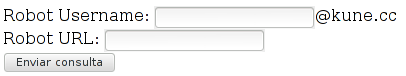
\includegraphics[keepaspectratio, scale=0.6]{Media/Captures/Wave/RegisterRobot.png}
  \caption{Robot Registration Screen}
  \label{fig:robot_register}
\end{figure}
In order to be able to interact with Wave it necessary to register the robot with the Wave server where the robot will be run. For example, for the Kune node kune.cc, go to \url{http://kune.cc/robot/register/create} and you will be prompted with the screen shown in Figure \ref{fig:robot_register}.\\[.2cm]
As username set the name you wish to give your robot, it should be a free name in the server, as names are unique. In the URL enter the URL where the gadget will be launched, it should be an URL reachable from within the Wave server. After sending the data you will receive a Consumer Token matching the name you entered, and a Consumer Token Secret: a secret key you will need to use to authenticate with OAuth and guarantee the identity of your robot.\\[.2cm]
There is no equivalent to the tester mode from GWT, but running a server for the robots is easy enough so that it is not a hassle. Using Maven plus Jetty in eclipse you can set the Maven goal to \verb|jetty:run| and the robot will be run.\\[.2cm]
Robots do basically two things: \textbf{Act when needed, and react to events}. Acting means modifying the documents, creating new blips, and more actions. And receiving events means a callback will be made to the robot when something from an external action happens on the Wave. The kind of events that are notified to the robot are the following:
\begin{itemize}
  \item WaveletBlipCreated: Triggered when a new blip is created.
  \item WaveletBlipRemoved: Triggered when a blip is deleted.
  \item WaveletParticipantsChanged: Triggered when a participant is added or removed.
  \item WaveletSelfAdded: Triggered when the own robot is added as a participant.
  \item WaveletSelfRemoved: Triggered when the own robot is removed as a participant.
  \item DocumentChanged: Triggered when the text of a document changes.
  \item AnnotatedTextChanged: Triggered when the annotations of a document change.
\end{itemize}
They are not compulsory but optional, \textbf{the developer can choose which events} will be transmitted. A public file called ``capabilities.xml'' has to be created in order to notify the Wave server of which events are implemented, and a hash is calculated based on those events to make it esaily visible when changes in how the robot acts have been made, because the hash will change.\\[.2cm]
There are other events documented such as GadgetStateChanged or WaveletTagsChanged, which even though available through the Robots API will not be triggered on the server, and therefore never received.
